\documentclass[lesson_slides]{subfiles}

\begin{document}
%%=-=-=-=-=-=-=-=-=-=-=-=-=-=-=-=-=-=-=-=-=-=-=-=-=-=-=-=-=-=-=-=-=-=-=-=-=-=-=-=
%   FRAME START   -=-=-=-=-=-=-=-=-=-=-=-=-=-=-=-=-=-=-=-=-=-=-=-=-=-=-=-=-=-=-=
\begin{frame}[c]{From predominant wh-ex situ to predominant wh-in situ}

\begin{columns}
    \column{0.5\textwidth}
        \centering
        \textbf{\textsc{the decline of wh-ex situ}}
    \begin{center}
        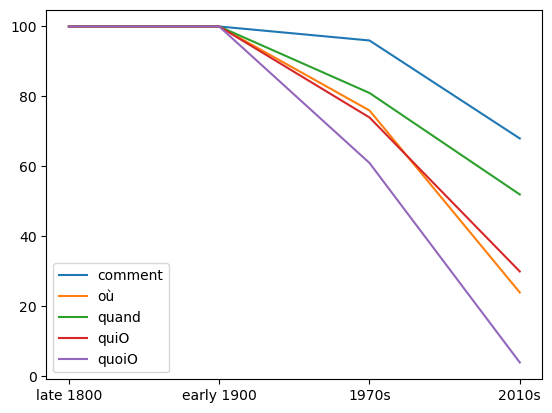
\includegraphics[width=\linewidth]{images/all.png}
    \end{center}
    \column{0.5\textwidth}
        \centering
        \textbf{\textsc{the rise of wh-in situ}}
        \begin{center}
        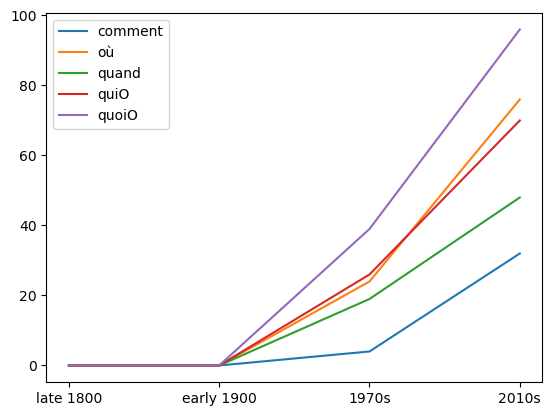
\includegraphics[width=\linewidth]{images/insitu.png}
    \end{center}
    \end{columns}
  
\end{frame}
%   FRAME END   --==-=-=-=-=-=-=-=-=-=-=-=-=-=-=-=-=-=-=-=-=-=-=-=-=-=-=-=-=-=-=
%=-=-=-=-=-=-=-=-=-=-=-=-=-=-=-=-=-=-=-=-=-=-=-=-=-=-=-=-=-=-=-=-=-=-=-=-=-=-=-=
\end{document}